\documentclass[11pt]{article}
\usepackage[spanish]{babel}
\usepackage{amsmath}
\usepackage{amssymb}
\usepackage{graphicx}
\graphicspath{ {./images/}, {~/Apunte/images/} }
\usepackage[utf8]{inputenc}
\usepackage[T1]{fontenc}
\usepackage[margin=1in]{geometry}
\usepackage{fancyhdr}
\usepackage{hyperref}

\hypersetup{
    pdftitle={Reporte Post-Laboratorio: Planillas de Cálculo 2},
    pdfauthor={Felipe Colli Olea},
    colorlinks=true,
    linkcolor=black,
    urlcolor=cyan
}

\pagestyle{fancy}
\fancyhf{}
\fancyfoot[C]{\footnotesize Felipe Colli, Todos los Derechos Reservados}
\fancyfoot[R]{\thepage}
\renewcommand{\headrulewidth}{0pt}

\title{Reporte Post-Laboratorio: Planillas de Cálculo 2 \\ \large{Herramientas Computacionales para Ingeniería y Ciencias}}
\author{Felipe Colli Olea}
\date{\today}

\begin{document}

\maketitle
\thispagestyle{fancy}

% ------------------------------------------------------------------------------
% INTRODUCCIÓN
% ------------------------------------------------------------------------------
\section{Introducción}

El presente informe expone el trabajo desarrollado durante el segundo laboratorio dedicado a las planillas de cálculo. Mientras que la sesión anterior se enfocó en el uso de referencias y operaciones aritméticas fundamentales, esta etapa introdujo herramientas analíticas de mayor complejidad algorítmica: la implementación manual de modelos de regresión estadística (Mínimos Cuadrados) y el uso de lógica condicional compuesta (\texttt{SI}, \texttt{Y}, \texttt{O}) para la agregación selectiva de datos.

Al igual que en las entregas anteriores, el enfoque de resolución priorizó la eficiencia matemática y la traducción de lógicas de programación convencionales hacia el paradigma funcional de celdas requerido por el software ofimático.

% ------------------------------------------------------------------------------
% DESARROLLO Y TRABAJOS REALIZADOS
% ------------------------------------------------------------------------------
\section{Desarrollo de Actividades}

\subsection{Problema 1: Análisis Macroeconómico y Regresión Lineal}
El primer problema consistió en analizar la correlación entre la tasa de desempleo ($X$) y el crecimiento económico ($Y$).

\begin{itemize}
	\item \textbf{Lógica Condicional (Análisis de Signos):} Se solicitó identificar los trimestres donde las variables presentaran un comportamiento inverso (distinto signo). En lugar de anidar múltiples condicionales, se optó por una optimización matemática aprovechando las propiedades de la multiplicación. La fórmula implementada fue \texttt{=SI(C2*D2 < 0; 1; 0)}, lo que reduce la evaluación lógica a una sola operación de comparación.

	\item \textbf{Modelo de Mínimos Cuadrados Ordinarios (OLS):} Se requirió calcular los parámetros de la recta de regresión lineal ($y = mx + c$) sin utilizar funciones predefinidas de estimación. Para ello, se construyeron las sumatorias $\sum X_i$, $\sum Y_i$, $\sum X_i^2$ y $\sum X_i Y_i$ vectorizando las columnas, y se implementaron las fórmulas matriciales para calcular la pendiente ($m$) y el coeficiente de posición ($c$). Finalmente, se contrastó la data real contra el modelo \texttt{mX+c} mediante un gráfico de dispersión multiserie.
\end{itemize}

% Placeholder para la imagen del Problema 1
\begin{figure}[h]
	\centering
	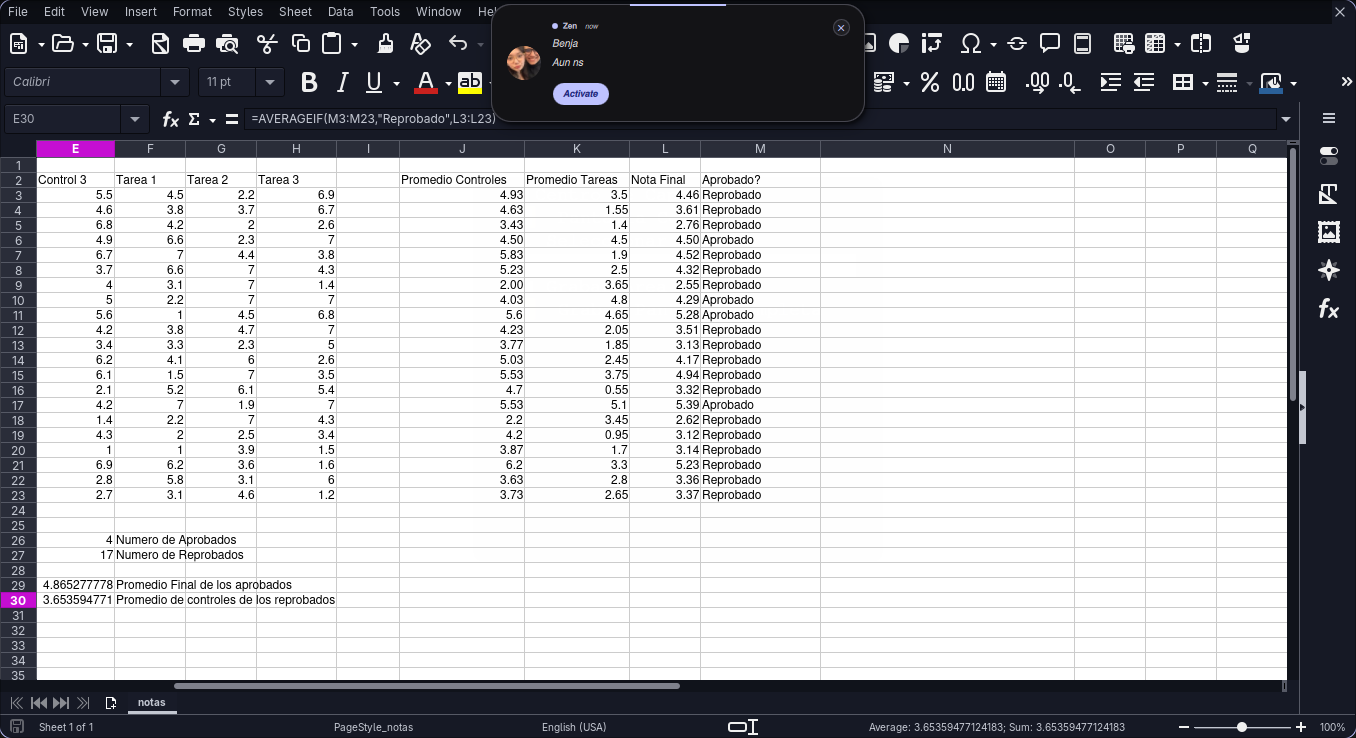
\includegraphics[width=0.8\textwidth]{nota.png}
	\caption{Cálculo manual de Mínimos Cuadrados y gráfico de regresión lineal.}
\end{figure}

\subsection{Problema 2: Automatización de Sistema de Calificaciones}
Esta actividad simuló la gestión académica de un curso, requiriendo el cálculo de promedios ponderados y la evaluación de criterios de aprobación estrictos.

\begin{itemize}
	\item \textbf{Manejo de Extremos (Descarte de notas):} Para calcular el promedio de tareas eliminando la peor calificación, se aplicó la fórmula \texttt{=(SUMA(F3:H3) - MIN(F3:H3))/2}. Este enfoque es algorítmicamente más robusto y escalable que ordenar y seleccionar manualmente las celdas.
	\item \textbf{Criterios Compuestos y Agregación:} La columna de estado académico requirió evaluar dos condiciones simultáneas utilizando operadores lógicos: \texttt{$=SI(Y(J3>5; K3>5); "Aprobado"; "Reprobado")$}. Posteriormente, se generaron métricas globales del curso mediante funciones de conteo y promedio condicional (\texttt{CONTAR.SI} y \texttt{PROMEDIO.SI}).
\end{itemize}

% Placeholder para la imagen del Problema 2
\begin{figure}[h]
	\centering
	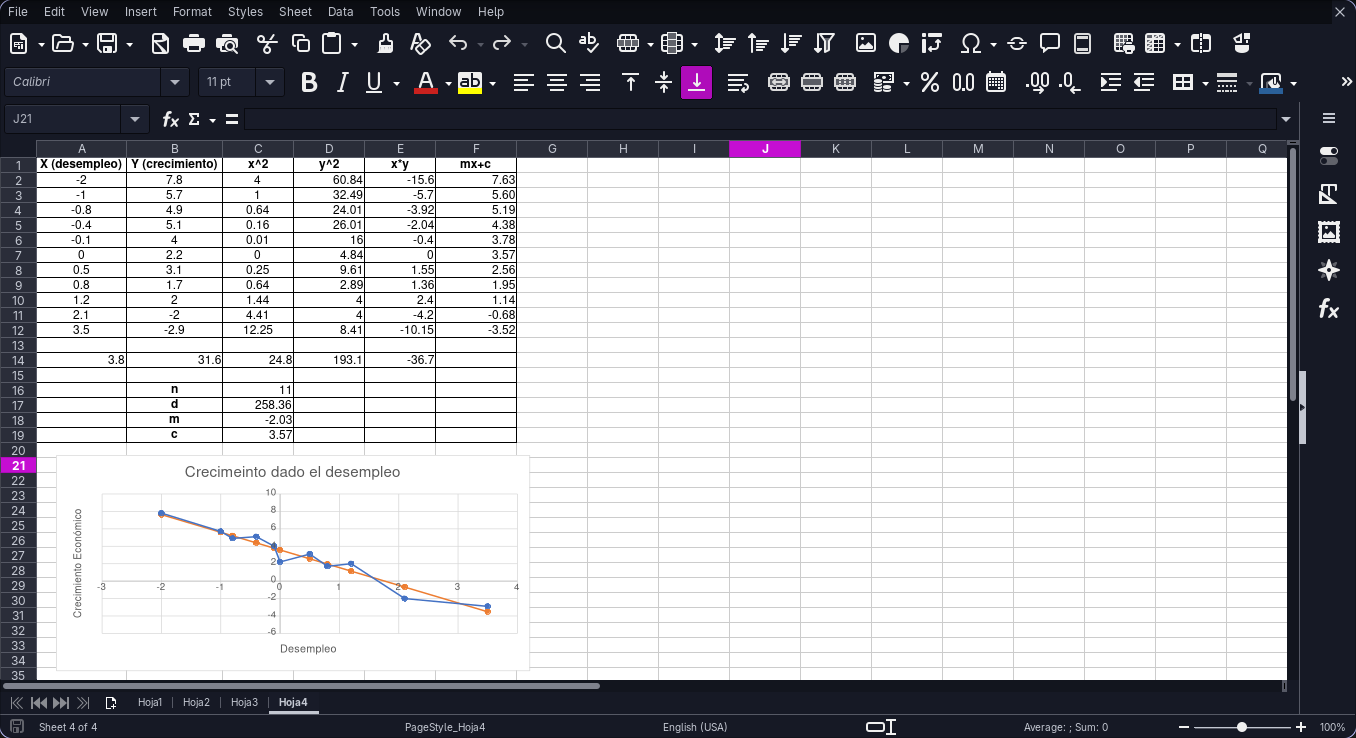
\includegraphics[width=0.8\textwidth]{reg.png}
	\caption{Sistema de calificaciones automatizado mediante lógica condicional.}
\end{figure}

\vspace{0.5cm}
\noindent\textit{\textbf{Nota sobre la evidencia visual:} Todo el desarrollo colaborativo y los cálculos fueron realizados en el entorno Windows/Excel de la facultad o mediante la plataforma Office365 online. No obstante, para mantener la coherencia de mi flujo de trabajo basado en código (Neovim/LaTeX), la compilación de este informe y la captura de las imágenes se efectuaron en mi estación de trabajo local bajo Arch Linux. Por consiguiente, las capturas de pantalla exponen la interfaz de \texttt{LibreOffice Calc}, el cual renderiza el archivo \texttt{.xlsx} con total fidelidad.}

\newpage
% ------------------------------------------------------------------------------
% REFLEXIONES Y DIFICULTADES
% ------------------------------------------------------------------------------
\section{Reflexiones y Dificultades}

Desde una óptica técnica, el laboratorio no impuso barreras analíticas, sino fricciones estructurales propias del lenguaje de fórmulas de las planillas.

La principal reflexión surge al comparar la implementación de Mínimos Cuadrados en este entorno versus un lenguaje de programación tradicional (como Python o R). En una planilla, la vectorización de operaciones (como multiplicar columnas para obtener $X \cdot Y$) obliga a crear columnas auxiliares físicas que saturan la interfaz visual, haciendo que el cálculo de parámetros como $d$, $m$ y $c$ dependa de múltiples celdas intermedias. En un entorno de \textit{Data Science} basado en código, este mismo proceso se resuelve en una sola línea mediante álgebra matricial o librerías optimizadas.

Asimismo, la implementación de la lógica condicional evidenció las limitaciones del encapsulamiento en celdas. Anidar múltiples funciones \texttt{SI()} o combinar compuertas lógicas \texttt{Y()}/\texttt{O()} genera bloques de "código" difíciles de leer, depurar (\textit{debuggear}) y mantener. La ausencia de indentación y saltos de línea estructurados hace que las planillas sean propensas a errores de sintaxis cuando las condiciones de negocio se vuelven complejas.

% ------------------------------------------------------------------------------
% CONCLUSIONES
% ------------------------------------------------------------------------------
\section{Conclusiones}

Este segundo laboratorio de planillas de cálculo consolidó el uso de herramientas estadísticas y lógicas para la toma de decisiones. Demostró que, incluso sin emplear módulos de programación avanzada como macros o VBA, es posible modelar relaciones bidimensionales completas y generar sistemas de evaluación automatizados.

A pesar de que las planillas ofimáticas carecen de la legibilidad, modularidad y control de versiones nativo que ofrecen los lenguajes de programación estructurados, su curva de aprendizaje casi nula y su capacidad de ofrecer \textit{feedback} visual instantáneo las mantiene como la herramienta de procesamiento de datos más ubicua de la industria. Entender sus lógicas de referenciación, funciones de agregación y limitaciones arquitectónicas es una competencia indispensable para el análisis preliminar de datos en la ingeniería.

\end{document}
